\subsection{A General Reaction-Diffusion Equation and its Weak Form}

The general form of a reaction-diffusion system is
\[
    \partial_t \mathbf{u} = \Gamma \nabla^2 \mathbf{u} + \mathbf{R} (\mathbf{u})
\]
where $\mathbf{u}(t, x, y)$ is a vector function describing the concentration of the reactants, $\Gamma$ is a diagonal matrix of diffusion coefficients, and $\mathbf{R}(\mathbf{u})$ is a potential nonlinear function describing the reactions between the reactants \parencite{martin1992nonlinear}. I solve the system on the domain $\Omega$ and assume the PDE has Neumann boundary conditions with derivative 0 for simplicity. The method could be extended to Neumann conditions with nonzero gradient across the boundary or Dirichlet conditions, but this is beyond the scope of this paper. Assuming the systems contains $N$ total reactions, each equation in the system is
\[
    \partial_t u_n = \gamma_n \nabla^2 u_n + r_n\left(\{u_m\}_{m = 1}^{N}\right), \quad n \in \{1, 2, \dots, N\}.
\]

The FEM solves for a solution to the weak form of the PDE \parencite{galerkin1968rods}. The weak form is given by multiplying by some function $v$ and integrating across the whole domain, which gets
\[
    \int_\Omega v \partial_t u_n dA = \int_\Omega v \left[ \gamma_n \nabla^2 u_n + r_n\left(\{u_m\}_{m = 1}^{N}\right)\right] dA.
\]
By the product rule for gradients and Neumann boundary conditions, we know
\[
    \int_\Omega v \gamma_n \nabla^2 u_n = -\gamma_n \int_\Omega \nabla v \cdot \nabla u_n dA.
\]
Therefore, the weak form is
\[
    \int_\Omega v \partial_t u_n dA = -\gamma_n \int_\Omega \nabla v \cdot \nabla u_n dA + \int_\Omega v r_n\left(\{u_m\}_{m = 1}^{N}\right) dA.
\]


\subsection{Discretization}

\begin{figure}[t!]
    \centering
    \caption{Triangulations of different domains}

    \begin{subfigure}{\textwidth}
        \centering
        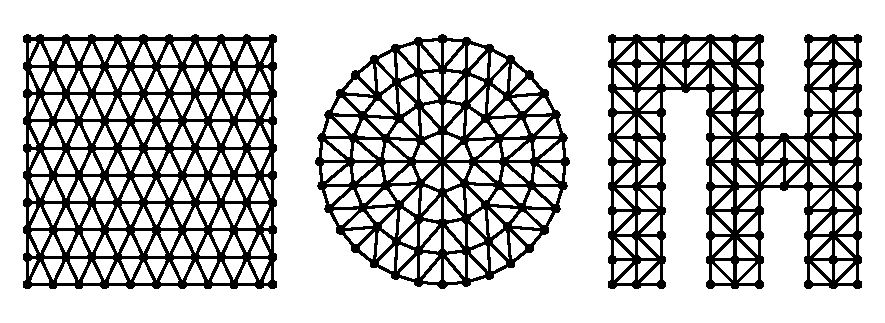
\includegraphics{figures/2dtris.pdf}
        \caption{2D Domains}
        \label{subfig:2dtris}
    \end{subfigure}

    \begin{subfigure}{\textwidth}
        \centering
        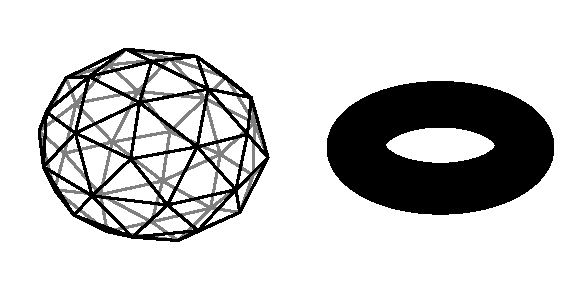
\includegraphics{figures/3dtris.pdf}
        \caption{3D Surface Domains}
        \label{subfig:3dtris}
    \end{subfigure}

    \label{fig:tris}
\end{figure}

To discretize the spacial derivative, I triangulate $\Omega$. Figure \ref{fig:tris} gives examples of what potential triangulations look like for a variety of domains. Panel \ref{subfig:2dtris} shows this discretization for 2D domains including a square, disk, and maze-like structure and Panel \ref{subfig:3dtris} shows this discretization along the surface of 3D objects, including a sphere and a torus.

For each vertex $v_i$ in the triangulation, I define a function $\psi_i$ such that
\begin{align*}
    \psi_i (v_i) &= 1 \\
    \psi_i (v_j) &= 0, \quad j \neq i
\end{align*}
and $\nabla \psi_i$ is constant along a triangle $T$. An example of $\psi_i$ for a vertex in the triangulation is in Figure \ref{fig:psi}. These functions will approximate the weak form of the PDE and the nonlinear reactions.

\begin{figure}[t!]
    \centering
    \caption{The function $\psi_i$ at a vertex}
    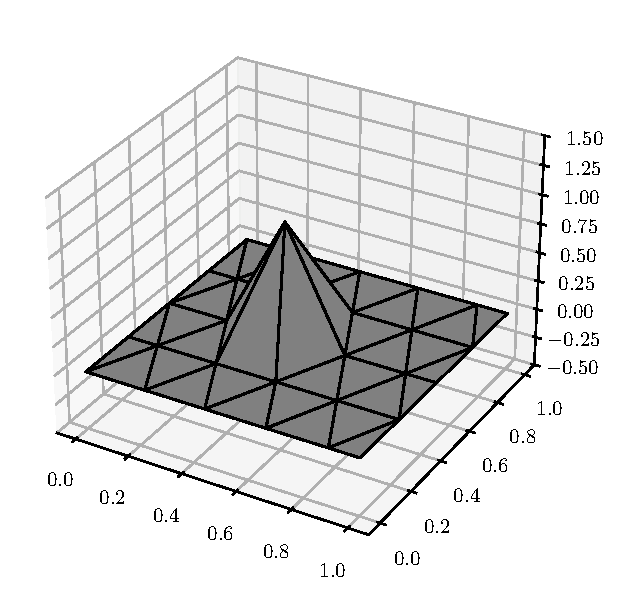
\includegraphics{figures/psi.pdf}
    \label{fig:psi}
\end{figure}

To discretize $u_n$, let $u_{n, i} (t)$ approximate $u(t, v_i)$. Then, we have
\[
    \hat{u}_n (t, x, y) = \sum_i \psi_i (x, y) u_{n, i} (t) \approx u(t, x, y).
\]
Similarly, we can approximate $r_n$ as
\[
    \hat{r}_n (t, x, y) = \sum_i \psi_i (x, y) r_n \left(\{u_{m, i} (t)\}_{m = 1}^N\right) \approx r_n(\{u_{m} (x, y, t)\}_{m = 1}^N).
\]
This approximation requires the solution for $u_n$ and $r_n$ to be adequately smooth across space and the triangulation to have a fine enough mesh. I analyze these assumptions in Section \ref{subsec:err} by solving systems with increasingly fine discretizations to get closer to the exact answer. Using these approximations and $v = \psi_i$ in the weak form gets
\[
    \sum_j \partial_t u_{n, j} \int_\Omega \psi_i \psi_j dA = -\gamma_n \sum_j u_{n, j} \int_\Omega \nabla \psi_i \cdot \nabla \psi_j dA + \sum_j r_n \left(\{u_{m, j} (t)\}_{m = 1}^N\right) \int_\Omega \psi_i \psi_j dA
\]
which represents the spatially discretized version of the system.

The temporal discretization is chosen to handle potential nonlinearities in the reaction function as well as maximize numerical stability. Specifically, I combine an explicit (forwards) Euler method to discretize the reaction step and an implicit (backwards) Euler method to discretize the diffusion step \parencite{sellami2020accelerating}. The explicit Euler step evaluates the reaction with known quantities to hangle nonlinearities before setting up a linear system, and the implicit Euler step maximizes the numerical stability of the solution \parencite{folland2020introduction}. Letting $u_{n, i}^t = u_{n, i}(t)$ at some discrete time step $t$, the time-discretized equation is
\[
    \sum_j u_{n, j}^t \left(\int_\Omega \psi_i \psi_j dA + \Delta t \gamma_n \int_\Omega \nabla \psi_i \cdot \nabla \psi_j dA\right) = \sum_j \left(u_{n, j}^{t - \Delta t} + \Delta t r_n \left(\{u_{m, j}^{t - \Delta t}\}_{m = 1}^N\right)\right) \int_\Omega \psi_i \psi_j dA.
\]


\subsection{Setting up a Linear System}

To solve the time-discretized equation, I turn it into a linear algebra problem. I define the damping matrix $\mathbf{D}$ so that
\[
    d_{i, j} = \int_\Omega \psi_i \psi_j dA
\]
and the stiffness matrix $\mathbf{S}$ so that
\[
    s_{i, j} = \int_\Omega \nabla \psi_i \cdot \nabla \psi_j dA.
\]
Since $d_{i, j} = 0$ and $s_{i, j} = 0$ whenever $v_i$ and $v_j$ don't share a triangle, the damping and stiffness matrices have a sparse structure that makes computation with them fast even on very fine triangulations of $\Omega$. Appendix \ref{app:mats} derives expressions for $d_{i, j}$ and $s_{i, j}$ in cases where $v_i$ and $v_j$ share at least one triangle.

Then, defining $\mathbf{u}_n^t$ as the vector with entries $u_{n, j}^t$, the equation becomes the linear system
\[
    \left(\mathbf{D} + \Delta t \gamma_n \mathbf{S}\right) \mathbf{u}_n^t = \mathbf{D} \left(\mathbf{u}_n^{t - \Delta t} + \Delta t r_n \left(\{\mathbf{u}_m^{t - \Delta t}\}_{m = 1}^N\right)\right)
\]
which allows me to solve for the solution at $t$ given a solution at time $t - \Delta t$. The function $r_n$ is vectorized and because $\mathbf{D} + \Delta t \gamma_n \mathbf{S}$ is sparse, symmetric, and positive-definite, I use the conjugate gradient method to solve for $\mathbf{u}_n^t$ \parencite{nazareth2009conjugate}. Together, this allows me to quickly solve for each time step.

Therefore, to solve the system I start with some initial condition $\mathbf{u}_n^0$ for each $n$. In the sections that follow, this initial condition is chosen to be random noise, although any initial condition could be used. Then, I solve the linearized version of the PDE for each $n$ to iterate to the next time step. Repeating this process to some final $T$ allows me to efficiently and accurately solve the reaction-diffusion PDE on any triangulated domain.
